%-*-latex-*-
\sectionthree{Heapify-down}
\begin{python0}
from solutions import *; clear()
\end{python0}

Heapify-down is the opposite of heapify-up:
you keep pushing a value \verb!v! down, swapping with the largest child
if that largest child is greater than \verb!v!. 
Here's an example.

Suppose I have this tree:

\begin{center}
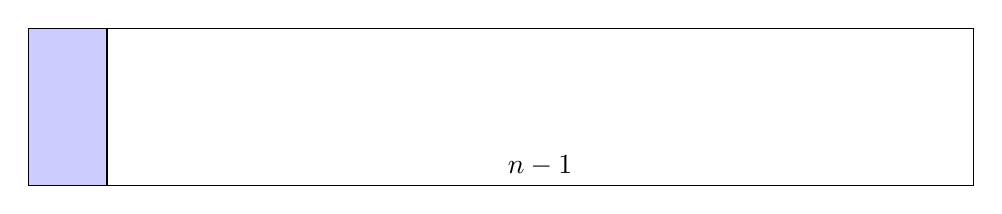
\begin{tikzpicture}

\draw (6.0, 1.0)
  node[draw, , , color=black,
       rounded corners=0cm, inner sep=0cm] {

\begin{minipage}[t][2cm]{12cm}
\mbox{}

\end{minipage}

};
\draw (0.5, 1.0)
  node[fill=blue!20!white,rounded corners=0cm,inner sep=0cm] {

\begin{minipage}[t][2cm]{1cm}
\mbox{}

\end{minipage}

};
\draw (0.5, 1.0)
  node[draw, , , color=black,
       rounded corners=0cm, inner sep=0cm] {

\begin{minipage}[t][2cm]{1cm}
\mbox{}

\end{minipage}

};
\draw (6.5, 0.25)
  node[draw=none, line width=0cm, , color=black,
       rounded corners=0cm, inner sep=0cm] {

\begin{minipage}[t][0.1cm]{0.1cm}
\mbox{}

\end{minipage}

};\draw (6.5, 0.25) node[color=black] {$n - 1$};
\end{tikzpicture}

\end{center}



This is almost a maxheap except that \verb!0!
violates the maxheap property.
I perform heapify-down at \verb!0!, swapping with
the larger of the children, i.e., \verb!5!


\begin{center}
\begin{tikzpicture}

\fill[blue!10] (0.0, 0.0) circle (0.3);
\node [line width=0.03cm,black,minimum size=0.57cm,draw,circle] at (0.0,0.0)(a){};\draw (0.0, 0.0) node[color=black] {$a$};
\fill[blue!10] (-2.0, -1.0) circle (0.3);
\node [line width=0.03cm,black,minimum size=0.57cm,draw,circle] at (-2.0,-1.0)(b){};\draw (-2.0, -1.0) node[color=black] {$b$};
\fill[blue!10] (2.0, -1.0) circle (0.3);
\node [line width=0.03cm,black,minimum size=0.57cm,draw,circle] at (2.0,-1.0)(d){};\draw (2.0, -1.0) node[color=black] {$d$};
\fill[blue!10] (-3.0, -2.0) circle (0.3);
\node [line width=0.03cm,black,minimum size=0.57cm,draw,circle] at (-3.0,-2.0)(e){};\draw (-3.0, -2.0) node[color=black] {$e$};
\fill[blue!10] (-1.0, -2.0) circle (0.3);
\node [line width=0.03cm,black,minimum size=0.57cm,draw,circle] at (-1.0,-2.0)(f){};\draw (-1.0, -2.0) node[color=black] {$f$};
\fill[blue!10] (1.0, -2.0) circle (0.3);
\node [line width=0.03cm,black,minimum size=0.57cm,draw,circle] at (1.0,-2.0)(h){};\draw (1.0, -2.0) node[color=black] {$h$};
\fill[blue!10] (3.0, -2.0) circle (0.3);
\node [line width=0.03cm,black,minimum size=0.57cm,draw,circle] at (3.0,-2.0)(o){};\draw (3.0, -2.0) node[color=black] {$o$};
\fill[blue!10] (-2.5, -3.0) circle (0.3);
\node [line width=0.03cm,black,minimum size=0.57cm,draw,circle] at (-2.5,-3.0)(l){};\draw (-2.5, -3.0) node[color=black] {$l$};
\fill[blue!10] (1.5, -3.0) circle (0.3);
\node [line width=0.03cm,black,minimum size=0.57cm,draw,circle] at (1.5,-3.0)(m){};\draw (1.5, -3.0) node[color=black] {$m$};
\fill[blue!10] (3.5, -3.0) circle (0.3);
\node [line width=0.03cm,black,minimum size=0.57cm,draw,circle] at (3.5,-3.0)(j){};\draw (3.5, -3.0) node[color=black] {$j$};\draw[line width=0.03cm,black,->,>=triangle 60] (a) to  (b);
\draw[line width=0.03cm,black,->,>=triangle 60] (a) to  (d);
\draw[line width=0.03cm,black,->,>=triangle 60] (b) to  (e);
\draw[line width=0.03cm,black,->,>=triangle 60] (b) to  (f);
\draw[line width=0.03cm,black,->,>=triangle 60] (d) to  (h);
\draw[line width=0.03cm,black,->,>=triangle 60] (d) to  (o);
\draw[line width=0.03cm,black,->,>=triangle 60] (e) to  (l);
\draw[line width=0.03cm,black,->,>=triangle 60] (h) to  (m);
\draw[line width=0.03cm,black,->,>=triangle 60] (o) to  (j);
\end{tikzpicture}

\end{center}



to get


\begin{center}
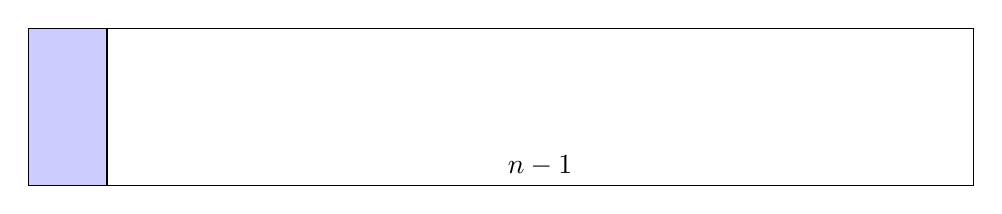
\begin{tikzpicture}

\draw (6.0, 1.0)
  node[draw, , , color=black,
       rounded corners=0cm, inner sep=0cm] {

\begin{minipage}[t][2cm]{12cm}
\mbox{}

\end{minipage}

};
\draw (0.5, 1.0)
  node[fill=blue!20!white,rounded corners=0cm,inner sep=0cm] {

\begin{minipage}[t][2cm]{1cm}
\mbox{}

\end{minipage}

};
\draw (0.5, 1.0)
  node[draw, , , color=black,
       rounded corners=0cm, inner sep=0cm] {

\begin{minipage}[t][2cm]{1cm}
\mbox{}

\end{minipage}

};
\draw (6.5, 0.25)
  node[draw=none, line width=0cm, , color=black,
       rounded corners=0cm, inner sep=0cm] {

\begin{minipage}[t][0.1cm]{0.1cm}
\mbox{}

\end{minipage}

};\draw (6.5, 0.25) node[color=black] {$n - 1$};
\end{tikzpicture}

\end{center}



I do it again, swapping \verb!0! with \verb!3! to get

\begin{center}
\begin{tikzpicture}

\fill[blue!10] (0.0, 0.0) circle (0.3);
\node [line width=0.03cm,black,minimum size=0.57cm,draw,circle] at (0.0,0.0)(a){};\draw (0.0, 0.0) node[color=black] {$a$};
\fill[blue!10] (-2.0, -1.0) circle (0.3);
\node [line width=0.03cm,black,minimum size=0.57cm,draw,circle] at (-2.0,-1.0)(b){};\draw (-2.0, -1.0) node[color=black] {$b$};
\fill[blue!10] (2.0, -1.0) circle (0.3);
\node [line width=0.03cm,black,minimum size=0.57cm,draw,circle] at (2.0,-1.0)(d){};\draw (2.0, -1.0) node[color=black] {$d$};
\fill[blue!10] (-3.0, -2.0) circle (0.3);
\node [line width=0.03cm,black,minimum size=0.57cm,draw,circle] at (-3.0,-2.0)(e){};\draw (-3.0, -2.0) node[color=black] {$e$};
\fill[blue!10] (-1.0, -2.0) circle (0.3);
\node [line width=0.03cm,black,minimum size=0.57cm,draw,circle] at (-1.0,-2.0)(f){};\draw (-1.0, -2.0) node[color=black] {$f$};
\fill[blue!10] (1.0, -2.0) circle (0.3);
\node [line width=0.03cm,black,minimum size=0.57cm,draw,circle] at (1.0,-2.0)(m){};\draw (1.0, -2.0) node[color=black] {$m$};
\fill[blue!10] (3.0, -2.0) circle (0.3);
\node [line width=0.03cm,black,minimum size=0.57cm,draw,circle] at (3.0,-2.0)(o){};\draw (3.0, -2.0) node[color=black] {$o$};
\fill[blue!10] (-3.5, -3.0) circle (0.3);
\node [line width=0.03cm,black,minimum size=0.57cm,draw,circle] at (-3.5,-3.0)(k){};\draw (-3.5, -3.0) node[color=black] {$k$};
\fill[blue!10] (-2.5, -3.0) circle (0.3);
\node [line width=0.03cm,black,minimum size=0.57cm,draw,circle] at (-2.5,-3.0)(l){};\draw (-2.5, -3.0) node[color=black] {$l$};
\fill[blue!10] (3.5, -3.0) circle (0.3);
\node [line width=0.03cm,black,minimum size=0.57cm,draw,circle] at (3.5,-3.0)(j){};\draw (3.5, -3.0) node[color=black] {$j$};\draw[line width=0.03cm,black,->,>=triangle 60] (a) to  (b);
\draw[line width=0.03cm,black,->,>=triangle 60] (a) to  (d);
\draw[line width=0.03cm,black,->,>=triangle 60] (b) to  (e);
\draw[line width=0.03cm,black,->,>=triangle 60] (b) to  (f);
\draw[line width=0.03cm,black,->,>=triangle 60] (d) to  (m);
\draw[line width=0.03cm,black,->,>=triangle 60] (d) to  (o);
\draw[line width=0.03cm,black,->,>=triangle 60] (e) to  (k);
\draw[line width=0.03cm,black,->,>=triangle 60] (e) to  (l);
\draw[line width=0.03cm,black,->,>=triangle 60] (o) to  (j);
\end{tikzpicture}

\end{center}



In this case, I stop at a leaf.
In general, it's possible that the heapify-down stops before
arriving at a leaf.

Note that I can heapify-down at any value even if
the tree has multiple spots that violate the
maxheap property.

\begin{Verbatim}[frame=single]
ALGORITHM: heapify-down (for maxheap)
INPUTS: x[0..n-1] -- array
        i         -- index of x

while i < n and x[i] has a child larger than x[i]:
    swap x[i] with the largest child, say x[j]
    set i to j
x[i] = val
\end{Verbatim}

In more details:

\begin{Verbatim}[frame=single]
ALGORITHM: heapify-down (for maxheap)
INPUTS: x[0..n-1] -- array
        i         -- index of x

v = x[i]
while 1:

    # Set j to index of the larger of the left and right
    # child of v. If there is no left and right child,
    # j is set to -1.
    l = left(i)
    r = right(i)
    if l == -1:
        # left child does no exist
        # (therefore right child does not exist)
        j = -1
    else:
        # left child exists
        if r == -1:
            # right child does not exists
            j = l
        else:
            # right child exists
            if x[l] > x[r]:
                j = l
            else:
                j = r    

    if j != -1 and x[j] > v:
        # v heapify-down                
        x[i] = x[j]
        i = j
    else:
        # v arrives at final index
        x[i] = v
        break
\end{Verbatim}

[REDUNDANT PARAGRAPH]
You can heapify-up or heapify-down at any index position.
There are times when heapifying-up or heapifying-down depends on the
value at the given index.
Let's call the function \verb!heapify!.
In such cases, if it's possible to heapify-up, then \verb!heapify! will
heapify-up and if it's possible to heapify-down, then \verb!heapify!
will heapify-down.

[What if there's a value that can heapify up and can heapify down?]


\begin{ex}
  In terms if actual real time, which cost more, one step of
  heapify-up or one step of heapify-down?
  \qed
\end{ex}
